\newpage
\section{Optimization models review}

% Scheduling
\subsection{Scheduling}

Nell'ambito dei problemi dello scheduling abbiamo degli elementi ben specificati:

\begin{itemize}
	\item \hl{task/job} già assegnati
	\item $n$ \hl{macchine/processori}
	\item potremmo attrezzare le macchine con dei \hl{tools}
\end{itemize}

Intendiamo \hl{allocare i tasks alla macchine in "overtime"} quindi capire anche la \hl{fascia temporale nella quale eseguire il task}. Potrebbe esserci un unico tempo di esecuzione oppure un task può avere dei tempi di esecuzione differenti su macchine differenti. 

L'output sarà un diagramma di Ganth.

\hl{I task possono avere degli istanti di rilascio} dove non potrebbe essere rilasciato dopo un certo istante di tempo (\hl{ready time}).

Possono esserci delle \hl{relazioni di precedenza tra i tasks}. Quindi non posso effettuare un task se prima non ho concluso l'altro.

Il diagramma mi dice nel tempo a che macchina è associato quale task ed in quali intervalli di tempo e con quale tool.


% Project scheduling
\subsection{Project scheduling}

Per progetto intendiamo un \hl{insieme di tasks che sono realizzati al fine di raggiungere un goal}. La caratteristica di un progetto è che nel complesso le attività non sono mai state eseguite in precedenza.

Le \hl{caratteristiche di un progetto} sono:


\begin{itemize}
	\item \textbf{durata delle attività} che nota
	\item ha \textbf{a capo un Project Manager}: responsabile del progetto e dei tempi di realizzazione, costi di produzione, ecc...
\end{itemize}

Un progetto è \hl{rappresentato da diverse attivita'} in una tabella fornita dal Project Manager:


\begin{table}[h!]
	\begin{center}
	\begin{tabular}{|c | c c |} 
			\hline
			Attività & Durata stimata $d_i$ & Predecessori \\ [0.5ex]
			\hline
 			1 & 10 & - \\
			2 & 10 & - \\
			3 & 10 & 1 \\
			4 & 10 & 1, 2 \\
			\hline
		\end{tabular}
	\end{center}
	\caption{Tabella di ore di lavoro e predecessioni delle attività}
	\label{tabatt}
\end{table}


e in un diagramma aciclico (Activity On Node (AoN)):


\begin{figure}[H]
\centering
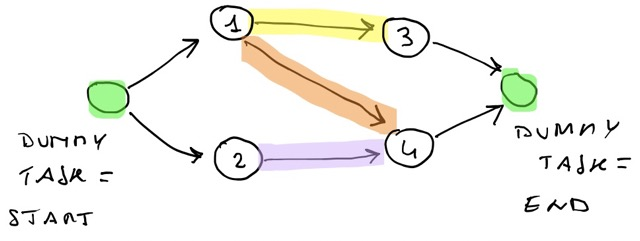
\includegraphics[scale=0.4]{aon.jpeg}
\caption{Diagramma Activity On Node} 
\label{aon}
\end{figure}


dove abbiamo degli "archi" che rappresentano le predecessioni. Avremo anche dei \hl{vertici fittizzi}:

\begin{itemize}
	\item start: lo colleghiamo tutte le attività che non hanno predecessori
	\item end: ci colleghiamo tutte le attività finali
\end{itemize}

Una funzione fondamentale del Project Manager è la possibilità di accelerare alcune attività agendo su:

\begin{itemize}
	\item \hl{Variabili decisionali}:
		
		nel nostro caso, è lo \hl{start time $s_i$}. Ipotizziamo che il progetto inizi al tempo $t = 0$, quindi per ogni task abbiamo che:

			$$s_i >= 0\ \ \ \forall\ \ \ i \in TASKS$$

		In più possiamo definire \hl{$T >= 0$ tempo di completamento del progetto} (\textbf{completion time}).

		Minimizziamo il completion time:

			$$\min z = T$$

		con $z = 1T + 0s_1 + 0s_2 + ... + 0s_n$
		
		
	\item \hl{relazioni di precedenza}:
	
		relazioni che portano alcuni nodi a dipendere da altri:
		
		$$
		p_{ij}=
		\begin{cases} 
		    1 \Leftrightarrow i \in j \\ 
		    0 altrimenti
		\end{cases}$$
		
		con \hl{$p_{ij}$ matrice} costate e binaria:
		
		$$p =
		\left[ {\begin{array}{cccc}
		    0 & 0 & 1 & 1 \\
			0 & 0 & 0 & 1 \\
		    0 & 0 & 0 & 0 \\
		    0 & 0 & 0 & 0 \\
		\end{array} } \right]$$
		
	
	\item \hl{vincoli di precedenza}:
	
		Sia \hl{$T$ maggiorante del tempo di completamento delle task}:
			$$s_i + d_i <= T$$

		allora:

			$$p_{ij} (s_i + d_i) <= s_j\ \ \ \forall\ \ \ i,j \in TASKS$$

		Possiamo avere che:

		\begin{itemize}
			\item \hl{$p_{ij} = 1$}: allora \textbf{$i$ è predecessore di $j$} quindi il tempo di inizio del task $j$ deve essere successivo o uguale al task $i$ cioè $s_i + d_i$
	
			\item \hl{$p_ij = 0$}: $i$ non è predecessore quindi avremo $0 <= s_j$ allora il vincolo è ridondante
		\end{itemize}
		
		scriviamo allora:
 
		$$s_i + d_i <= s_j\ \ \ \forall\ \ \ i,j \in TASKS,\ p_{ij} >= 0$$


\end{itemize}


% Esempio
\subsection{Esempio }

Un modello espanso per problemi di istanza:

\begin{enumerate}
	\item funzione obiettibo: $\min z = T$
	\item vincoli:
		\begin{itemize}
			\item $s_1 + 10 <= T$
			\item $s_2 + 10 <= T$
			\item $s_3 + 10 <= T$
			\item $s_4 + 10 <= T$
			\item $s_1 + 10 <= s_3 (p_{13} = 1)$
			\item $s_1 + 10 <= s_4 (p_{14} = 1)$
			\item $s_2 + 10 <= s_4 (p_{24} = 1)$
			\item $s_1, s_2, s_3, s_4 >= 0$
			\item $T >= 0$
		\end{itemize}
\end{enumerate}


% Velocizzazione del progetto
\subsection{Velocizzazione del progetto}

Il Project Manager ha un \hl{budget} per poter velocizzare il progetto.

Se considero un \hl{task $i$ con durata non costante ($d_i^N$)}, avremo un valore nominale che dipende da un budget extra.

Il più semplice è l'\hl{andamento lineare} dove all'aumentare delle risorse la durata si riduce in modo lineare. Il che è vero finché non si incontra un \hl{vincolo inferiore $d_i^m$}.


Le \hl{3 risorse} alle quali si possono far riferimento sono le \hl{3M}:

\begin{itemize}
	\item Man
	\item Machine
	\item Money
\end{itemize}


quindi $d_i = d_i^N$.


\begin{figure}[H]
\centering
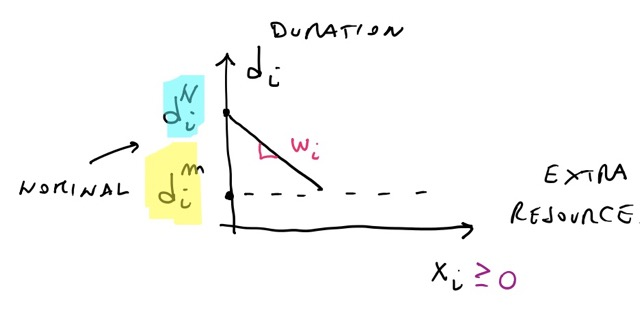
\includegraphics[scale=0.4]{budget.jpeg}
\caption{Diagramma budget} 
\label{budget}
\end{figure}


con:

\begin{itemize}
	\item \hl{pendenza w}: \textbf{riduzione della durata del task $i$} per unità di extra risorse (mesi di lavoro / k euro)
	\item $d_i = d_i^N - w_i x_i >= d_i^m$ vincolo del valore minimo per task
	\item $x_i$: denaro usato per il task $i$
	\item $B$: budget totale

\end{itemize}


% Esempio velocizzazione progetto
\subsection{Esempio velocizzazione progetto}

Avremo un modello con:

\begin{enumerate}
	\item funzione obiettivo: $\min z = T$
	\item vincoli:
		
		\begin{itemize}
			\item $s_i + d_i^N - w_i x_i <= T\ \ \ \forall\ \ \ i \in TASKS$
			\item $s_i + d_i^N - w_i x_i <= s_j\ \ \ \forall\ \ \ i, j \in TASKS, p_{ij} = 1$
			\item $d_i^N - w_i x_i >= d_i^m\ \ \ \forall\ \ \ i \in TASKS$
			\item $\sum_{i \in TASKS} x_i <= B$
			\item $T >= 0$
			\item $s_i >= 0\ \ \ \forall\ \ \ i \in TASKS$
			\item $x_i >= 0\ \ \ \forall\ \ \ i \in TASKS$
		\end{itemize}
\end{enumerate}


% Low sizing models
\subsection{Low sizing models}

Sono in genere usati da aziende manifatturiere. 


\begin{figure}[H]
\centering
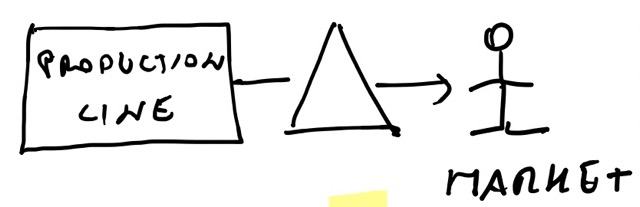
\includegraphics[scale=0.3]{prodline.jpeg}
\caption{Processo produtivo} 
\label{procprod}
\end{figure}


Supponendo di avere un \hl{tasso di domanda $d$} costante in base al tipo di prodotto. Ogni tipo di prodotto si differenzia dagli altri con una piccola modifica come può essere un differente gusto per una produzione di yogurt.

Questa differenziazione porta ad un \hl{costo di setup} delle macchine che andranno pulite, generando un costo fisso $k$.

Il livello di scorte sarà rappresentato con dei picchi con ampiezza $q$:


\begin{figure}[H]
\centering
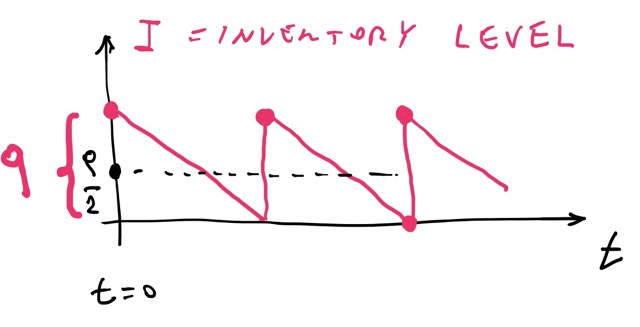
\includegraphics[scale=0.3]{invlev.jpeg}
\caption{Livello di inventario} 
\label{invlev}
\end{figure}


avendo una domanda costante, avremo una diminuzione lineare nello scorte di magazzino.

Ovviamente avremo dei \hl{costi medi di stockaggio $h$} dato che le scorte si "muoveranno" scambiandosi con altre scorte che entrano nel magazzino. Quindi andremo a calcolare il costo in base alla giacenza del \hl{numero di scorte medie $\frac{q}{2}$}.

In base alla strategia avremo:

\begin{enumerate}
	\item \hl{caso estermo}:
	
		gestione di tipo \textbf{just in time} dove \textbf{produco solo sotto commissione del cliente}.

		Avremo quindi:
		
		\begin{itemize}
			\item \textbf{livello di scorte molto basso} con un livello medio delle scorte molto basso e dei \textbf{costi di stockaggio bassi}
			\item \textbf{maggioramento dei costi del setup}
			\item pago $k$ più volte durante l'anno
		\end{itemize}
		
	\item \hl{caso produzione annua}:
	
		si produce un \textbf{quantitativo pari alla domanda annua}.
		
		Avremo quindi:
		
		\begin{itemize}
			\item grandi \textbf{costi di stockaggio}
			\item pago $k$ solo una volta all'anno
		\end{itemize}

\end{enumerate}


\begin{figure}[H]
\centering
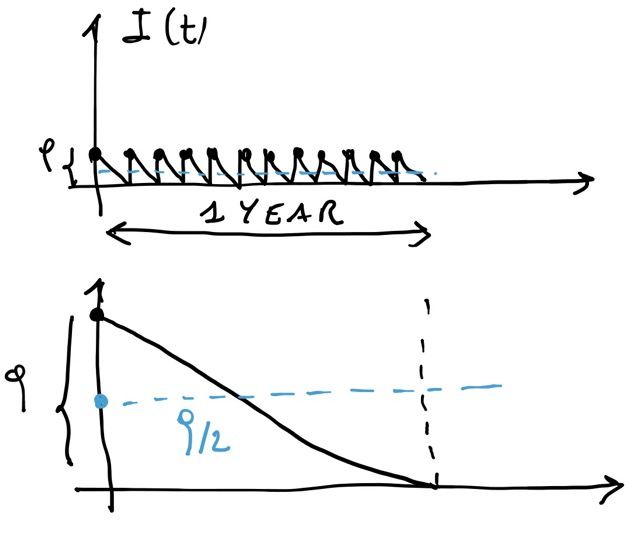
\includegraphics[scale=0.3]{casipart.jpeg}
\caption{Casi particolari} 
\label{casipart}
\end{figure}


% Scrivere il modello di ottimizzazione
\subsection{Scrivere il modello di ottimizzazione}

Le fasi da seguire prevedono la scrittura di:

\begin{enumerate}
	\item \hl{variabili decisionali}: variabile matematica per descrivere la mia decisione
	\item \hl{funzione obiettivo}: costo totale annuale composto dal \textbf{costo di scorta e quello di setup}
\end{enumerate}

Avremo allora:

$$z = k \frac{d}{q} + h \frac{q}{2} $$


Per la \hl{soluzione ottima}, faccio il gradiente:

$$\frac{dz}{dq} = 0 \Leftrightarrow -k \frac{d}{q^2} + \frac{h}{2} = 0$$


Concludiamo che il \hl{lotto economico}, per minimizzare i costi, sarà raggiunto da:

$$q^* = \sqrt{\frac{2kd}{h}}$$


\begin{figure}[H]
\centering
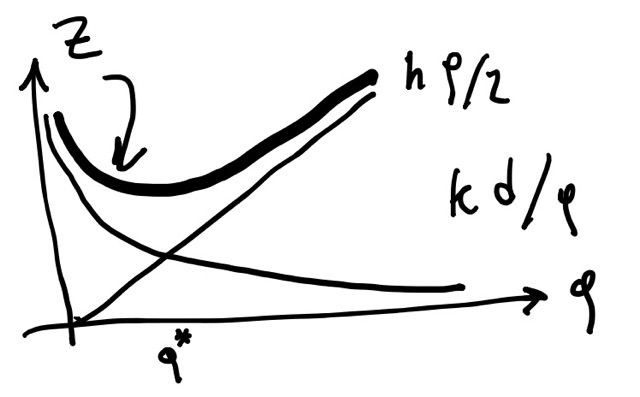
\includegraphics[scale=0.3]{lottoec.jpeg}
\caption{Caso di lotto economico} 
\label{lottoec}
\end{figure}
